%------------------------ Literature ------------------------

\chapter{کارهای پیشین}
در فصل سوم پایان‌نامه، کارهای پیشین انجام‌شده روی مساله به تفصیل توضیح داده می‌شود. نمونه‌ای از فصل کارهای پیشین\footnote{مطالب این فصل نمونه از پایان‌نامه‌ی آقای بهنام حاتمی گرفته شده است.} در زیر آمده است.


\section{مساله‌های خوشه‌بندی}
مساله‌ی \textbf{خوشه‌بندی}\LTRfootnote{Clustering} یکی از مهم‌ترین مسائل در زمینه‌ی داده‌کاوی به حساب می‌آید. در این مساله، هدف دسته‌بندی تعدادی شی به‌گونه‌ای است که اشیا درون یک دسته (خوشه)، نسبت به یکدیگر در برابر دسته‌های دیگر شبیه‌تر باشند (معیارهای متفاوتی برای تشابه تعریف می‌گردد). این مساله در حوزه‌های مختلفی از علوم کامپیوتر از جمله داده‌کاوی، جست‌وجوی الگو\LTRfootnote{Pattern Recognition} پردازش تصویر\LTRfootnote{Image Analysis}، بازیابی اطلاعات\LTRfootnote{Information Retrieval} و رایانش زیستی\LTRfootnote{Bioinformatics} مورد استفاده قرار می‌گیرد \cite{han2006}.

تا کنون راه‌حل‌های زیادی برای این مساله ارایه شده است که از لحاظ معیار تشخیص خوشه‌ها و نحوه‌ی انتخاب یک خوشه، با یک‌دیگر تفاوت بسیاری دارند. به همین خاطر مساله‌ی خوشه‌بندی یک مساله‌ی بهینه‌سازی چندهدفه\LTRfootnote{Multi-Objective Optimization} محسوب می‌شود.

همان طور که در مرجع \cite{estivill2002so} ذکر شده است، خوشه در خوشه‌بندی تعریف واحدی ندارد و یکی از دلایل وجود الگوریتم‌های متفاوت، همین تفاوت تعریف‌ها از خوشه است. بنابراین با توجه به مدلی که برای خوشه‌ها ارایه می‌شود، الگوریتم متفاوتی نیز ارایه می‌گردد. در ادامه به بررسی تعدادی از معروف‌ترین مدل‌های مطرح می‌پردازیم.
\begin{itemize}
\item \textbf{مدل‌های مرکزگرا}:
در این مدل‌ها، هر دسته با یک مرکز نشان داده می‌شود. از جمله معروف‌ترین روش‌های خوشه‌بندی بر اساس این مدل،  خوشه‌بندی $k$-مرکز، خوشه‌بندی $k$-میانگین\LTRfootnote{$k$-Means} و خوشه‌بندی $k$-میانه\LTRfootnote{$k$-Median} است.
\item \textbf{مدل‌های مبتنی بر توزیع نقاط}:
در این مدل‌ها، دسته‌ها با فرض پیروی از یک توزیع احتمالی مشخص می‌شوند. از جمله الگوریتم‌های معروف ارایه شده در این مدل، الگوریتم بیشینه‌سازی امید ریاضی \LTRfootnote{Expectation Maximization} است.
\item \textbf{مدل‌های مبتنی بر تراکم نقاط}:
در این مدل‌ها، خوشه‌ها متناسب با ناحیه‌های متراکم نقاط در مجموعه داده مورد استفاده قرار می‌گیرد.
\item \textbf{مدل‌های مبتنی بر گراف}:
در این مدل‌ها، هر خوشه به مجموعه از راس‌ها گفته می‌شود که تمام راس‌های آن با یک‌دیگر همسایه باشند.از جمله الگوریتم‌های معروف این مدل، الگوریتم خوشه‌بندی \lr{HCS}\LTRfootnote{Highly Connected Subgraphs} است.
\end{itemize}

الگوریتم‌های ارایه شده تنها از نظر نوع مدل با یک‌دیگر متفاوت نیستند بلکه، می‌توان آن‌ها را از لحاظ نحوه‌ی تخصیص نقاط بین خوشه‌ها نیز تقسیم‌بندی کرد.
\begin{itemize}
\item \textbf{تخصیص قطعی داده‌ها}:
در این نوع خوشه‌بندی هر داده دقیقاً به یک خوشه اختصاص داده می‌شود.
\item \textbf{تخصیص قطعی داده‌ها با داده‌ی پرت}:
در این نوع خوشه‌بندی ممکن است بعضی از داده‌ها به هیچ خوشه‌ای اختصاص نیابد، اما بقیه داده‌ها هر کدام دقیقاً به یک خوشه اختصاص می‌یابد.
\item \textbf{تخصیص قطعی داده}:
در این نوع خوشه‌بندی هر داده دقیقاً به یک خوشه اختصاص داده می‌شود.
\item \textbf{خوشه‌بندی هم‌پوشان}:
در این نوع خوشه‌بندی هر داده می‌تواند به چند خوشه اختصاص داده شود. در گونه‌ای از این مدل، می‌توان هر نقطه را با احتمالی به هر خوشه اختصاص می‌یابد. به این گونه از خوشه‌بندی، خوشه‌بندی نرم\LTRfootnote{Soft Clustering} گفته می‌شود.
\item \textbf{خوشه‌بندی سلسه‌مراتبی}:
در این نوع خوشه‌ها، داده‌ها به گونه‌ای به خوشه‌ها تخصیص داده می‌شود که دو خوشه یا اشتراک ندارند یا یکی به طور کامل دیگری را می‌پوشاند. در واقع در بین خوشه‌ها، رابطه‌ی پدر فرزندی برقرار است.
\end{itemize}

در بین دسته‌بندی‌های ذکر شده، تمرکز اصلی این پایان‌نامه بر روی مدل مرکزگرا و خوشه‌بندی قطعی با داده‌های پرت با مدل $k$-مرکز است. همان‌طور که ذکر شد علاوه بر مساله‌ی $k$-مرکز که به تفصیل مورد بررسی قرار می‌گیرد، $k$-میانه و $k$-میانگین از جمله معروف‌ترین خوشه‌بندی‌های مدل مرکزگرا هستند. در خوشه‌بندی $k$-میانه، هدف افراز نقاط به $k$ خوشه است به گونه‌ای که مجموع مربع فاصله‌ی هر نقطه از میانه‌ی نقاط آن خوشه، کمینه گردد. در خوشه‌بندی $k$-میانگین، هدف افراز نقاط به $k$ خوشه است به گونه‌ای که مجموع فاصله‌ی هر نقطه از میانگین نقاط داخل خوشه (یا مرکز آن خوشه) کمینه گردد. 

\section{خوشه‌بندی $k$-مرکز}
یکی از رویکردهای شناخته‌شده برای مساله‌ی خوشه‌بندی، مساله‌ی \textbf{$\boldsymbol{k}$-مرکز} است. در این مساله هدف، پیدا کردن $k$ نقطه به عنوان مرکز دسته‌ها است به طوری که شعاع دسته‌ها تا حد ممکن کمینه شود. مثالی از مساله‌ی $2$-مرکز در شکل \ref{fig:two:center} نشان داده شده است. در این پژوهش، مساله‌ی $k$-مرکز با متریک‌های خاص و برای $k$های کوچک مورد بررسی قرار گرفته است و هر کدام از‌ تعریف رسمی مساله‌ی $k$-مرکز در زیر آمده است.

\begin{figure}[b!]
\centering
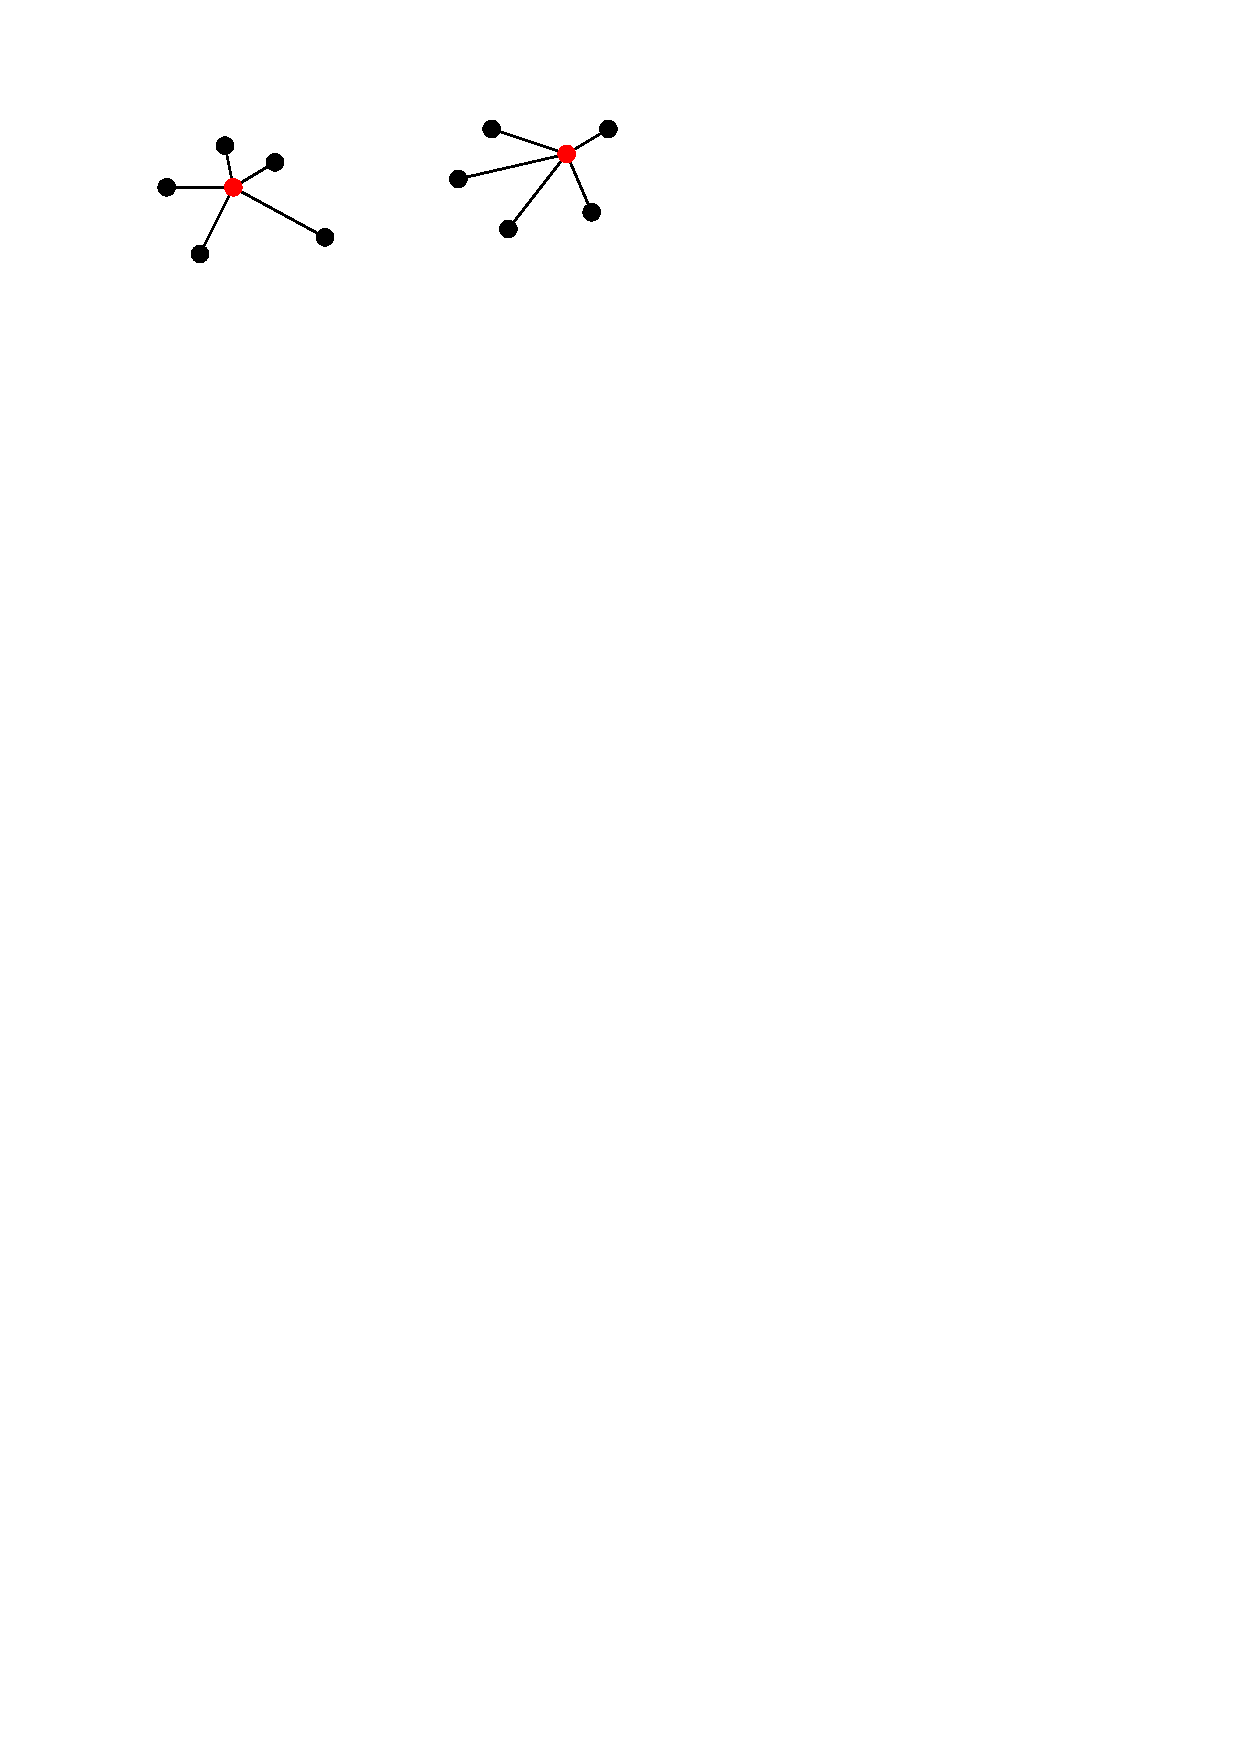
\includegraphics[width=8cm]{k-center}
\caption{نمونه‌ای از ‌مساله‌ی ۲-مرکز}
\label{fig:two:center}
\end{figure}

\begin{prb}[$k$-مرکز]
گراف کامل بدون جهت $G = (V, E)$ با تابع فاصله‌ی $d$، که از نامساوی مثلثی پیروی می‌کند داده ‌شده است. زیرمجموعه‌ی $S \subseteq V$ با اندازه‌ی $k$ را به گونه‌ای انتخاب کنید که عبارت زیر را کمینه کند.
\begin{equation}
\max_{v \in V} \min_{s \in S} d(v, s)
\end{equation}
\end{prb}

گونه‌های مختلفی از مساله‌ی $k$-مرکز با محدودیت‌های متفاوت توسط پژوهشگران مورد مطالعه قرار گرفته است. از جمله‌ی این گونه‌ها، می‌توان به حالتی که در بین داده‌های ورودی، داده‌های پرت وجود دارد، اشاره کرد. در واقع در این مساله، قبل از خوشه‌بندی می‌توانیم تعدادی از نقاط ورودی را حذف نموده و سپس به خوشه‌بندی نقاط بپردازیم. سختی این مساله از آنجاست که نه تنها باید مساله‌ی خوشه‌بندی را حل نمود، بلکه در ابتدا باید تصمیم گرفت که کدام یک از داده‌ها را به‌عنوان داده‌ی پرت در نظر گرفت که بهترین جواب در زمان خوشه‌بندی به دست آید. در واقع اگر تعداد نقاط پرتی که مجاز به حذف است، برابر صفر باشد، مساله به مساله‌ی $k$-مرکز تبدیل می‌شود. نمونه‌ای از مساله‌ی $2$-مرکز با $7$ داده‌ی پرت را در شکل \ref{fig:two:center:outlier} می‌توانید ببینید. تعریف دقیق‌تر این مساله در زیر آمده است.

\begin{prb}[$k$-مرکز با داده‌های پرت]
یک گراف کامل بدون جهت $G = (V, E)$ با تابع فاصله‌ی $d$، که از نامساوی مثلثی پیروی می‌کند داده‌شده است. زیرمجموعه‌ی $Z \subseteq V$ با اندازه‌ی $z$ و  مجموعه‌ی $S \subseteq V - Z$ با اندازه‌ی $k$ را انتخاب کنید به‌ طوری ‌که عبارت زیر را کمینه کند.
\begin{equation}
\max_{v \in V - Z} \min_{s \in S} d(v, s)
\end{equation}
\end{prb}

\begin{figure}[b!]
\centering
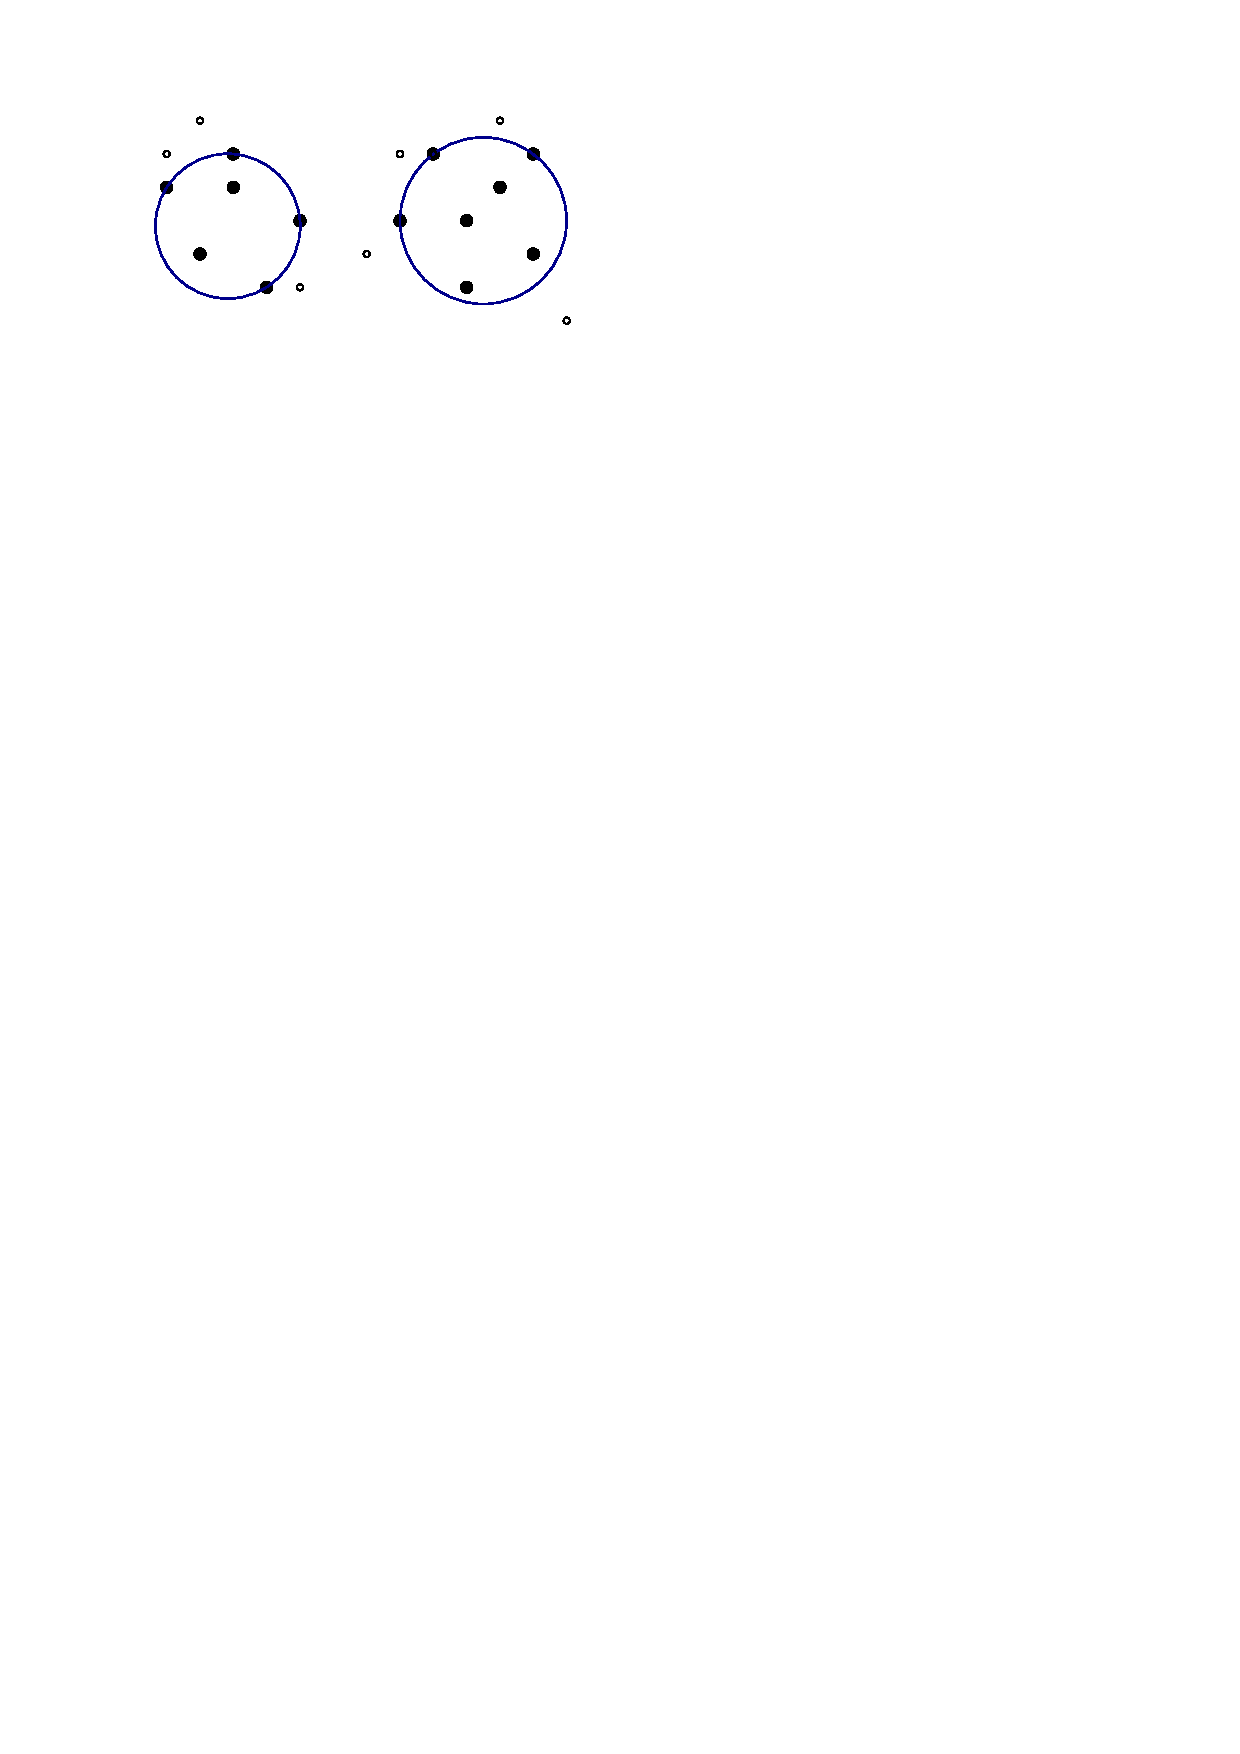
\includegraphics[width=8cm]{outlier}
\caption{نمونه‌ای از‌مساله‌ی ۲-مرکز با داده‌های پرت}
\label{fig:two:center:outlier}
\end{figure}

گونه‌ی دیگری از مساله‌ی $k$-مرکز که در سال‌های اخیر مورد توجه قرار گرفته است، حالت جویبار داده‌ی آن است. در این‌گونه از مساله‌ی $k$-مرکز، در ابتدا تمام نقاط در دسترس نیستند، بلکه به‌مرور زمان نقاط در دسترس قرار می‌گیرند. محدودیت دومی که وجود دارد، محدودیت حافظه است، به طوری که نمی‌توان تمام نقاط را در حافظه نگه داشت و بعضاً حتی امکان نگه‌داری در حافظه‌ی جانبی نیز وجود ندارد و به‌طور معمول باید مرتبه‌ی حافظه‌ای کم‌تر از مرتبه حافظه‌ی \textbf{خطی}\LTRfootnote{Linear} متناسب با تعداد نقاط استفاده نمود. از این به بعد به چنین مرتبه‌ای، مرتبه‌ی \textbf{زیرخطی}\LTRfootnote{Sublinear} می‌گوییم. مدلی که ما در این پژوهش بر روی آن تمرکز داریم مدل جویبار داده تک‌گذره \LTRfootnote{Single pass}\cite{aggarwal2007data} است. یعنی تنها یک بار می‌توان از ابتدا تا انتهای داده‌ها را بررسی کرد و پس از عبور از یک داده، اگر آن داده در حافظه ذخیره نشده باشد، دیگر به آن دسترسی وجود ندارد. علاوه بر این، در هر لحظه باید بتوان به پرسمان (برای تمام نقاطی از جویبار داده که تاکنون به آن دسترسی داشته‌ایم) پاسخ داد.

\begin{prb}[$k$-مرکز در حالت جویبار داده]
مجموعه‌ای از نقاط در فضای $d$-بعدی به مرور زمان داده می‌شود. در هر لحظه از زمان، به ازای مجموعه‌ی $U$ از نقاطی که تا کنون وارد شده‌اند، زیرمجموعه‌ی $S \subseteq U$ با اندازه‌ی $k$ را انتخاب کنید به ‌طوری ‌که عبارت زیر کمینه شود.
\begin{equation}
\max_{u \in U} \min_{s \in S} d(u, s)
\end{equation}
\end{prb}

از آنجایی که گونه‌ی جویبار داده و داده پرت مساله‌ی $k$-مرکز به علت به‌روز بودن مبحث داده‌های حجیم\LTRfootnote{Big Data}، به تازگی مورد توجه قرار گرفته است. در این تحقیق سعی شده است که تمرکز بر روی این‌گونه‌ی خاص از مساله باشد. همچنین در این پژوهش سعی می‌شود گونه‌های مساله را برای انواع متریک‌ها و برای $k$های کوچک نیز مورد بررسی قرار داد. 

\section{مدل جویبار داده}
همان‌طور که ذکر شد مساله‌ی $k$-مرکز در حالت داده‌های پرت و جویبار داده، گونه‌های تعمیم‌یافته از مساله‌ی $k$-مرکز هستند و در حالت‌های خاص به مساله‌ی $k$-مرکز کاهش پیدا می‌کنند. مساله‌ی $k$-مرکز در حوزه‌ی مسائل ان‌پی-سخت\LTRfootnote{NP-Hard} قرار می‌گیرد و با فرض $P \neq NP$ الگوریتم دقیق با زمان چندجمله‌ای برای آن وجود ندارد \cite{michael1979computers}. بنابراین برای حل کارای\LTRfootnote{Efficient} این مسائل از الگوریتم‌های تقریبی\LTRfootnote{Approximation Algorithm} استفاده می‌شود.

برای مساله‌ی $k$-مرکز، دو الگوریتم تقریبی معروف وجود دارد. در الگوریتم اول، که به روش حریصانه\LTRfootnote{Greedy} عمل می‌کند، در هر مرحله بهترین مرکز ممکن را انتخاب می‌کند به طوری تا حد ممکن از مراکز قبلی دور باشد \cite{megiddo1984complexity}. این الگوریتم، الگوریتم تقریبی با ضریب تقریب 2 ارایه می‌دهد. در الگوریتم دوم، با استفاده از مساله‌ی مجموعه‌ی غالب کمینه\LTRfootnote{Dominating Set}، الگوریتمی با ضریب تقریب ۲ ارایه می‌گردد \cite{vazirani2013approximation}. همچنین ثابت شده است، که بهتر از این ضریب تقریب، الگوریتمی نمی‌توان ارایه داد مگر آن‌که $P = NP$ باشد.

برای مساله‌ی $k$-مرکز در حالت جویبار داده برای ابعاد بالا، بهترین الگوریتم موجود ضریب تقریب $2 + \eps$ دارد \cite{mccutchen2008streaming, guha2009tight, ahn2014computing} و ثابت می‌شود الگوریتمی با ضریب تقریب بهتر از $2$ نمی‌توان ارایه داد. برای مساله‌ی $k$-مرکز با داده‌ی پرت در حالت جویبار داده نیز، بهترین الگوریتم ارایه شده، الگوریتمی با ضریب تقریب $4 + \eps$ است که با کران پایین $3$ هنوز اختلاف قابل توجهی دارد \cite{charikar2001algorithms}. 

برای $k$ های کوچ به خصوص $k =1, 2$، الگوریتم‌های بهتری ارایه شده است. بهترین الگوریتم ارایه شده برای مساله‌ی $1$-مرکز در حالت جویبار داده برای ابعاد بالا، دارای ضریب تقریب $1.22$ است و کران پایین $\frac{1 + \sqrt{2}}{2}$ نیز برای این مساله اثبات شده است \cite{agarwal2010streaming, chan2014streaming}. برای مساله $2$-مرکز در حالت جویبار داده برای ابعاد بالا، اخیرا راه‌حلی با ضریب تقریب $1.8 + \eps$ ارایه شده است \cite{kim2014improved}. برای مساله‌ی $1$-مرکز با داده‌ی پرت، تنها الگوریتم موجود، الگوریتمی با ضریب تقریب $1.73$ است \cite{zarrabi2009streaming}.

\section{تقریب‌پذیری}
یکی از راه‌کارهایی که برای کارآمد کردن راه‌حل ارایه شده برای یک مساله وجود دارد، استفاده از الگوریتم‌های تقریبی برای حل آن مساله است. یکی از عمده‌ترین دغدغه‌های مطرح در الگوریتم‌های تقریبی کاهش ضریب تقریب است. در بعضی از موارد حتی امکان ارایه‌ی الگوریتم تقریبی با ضریبی ثابت نیز وجود ندارد. به طور مثال، الگوریتم تقریبی با ضریب تقریب کم‌تر از $2$، برای مساله‌ی $k$-مرکز وجود ندارد مگر این‌که $\mathsf{P} = \mathsf{NP}$ باشد. برای مسائل مختلف، معمولاً می‌توان کران پایینی برای میزان تقریب‌پذیری آن‌ها ارایه داد. در واقع برای برخی مسائل ان‌پی-سخت، علاوه بر این که الگوریتم کارآمدی وجود ندارد، گاهی الگوریتم تقریبی با ضریبی تقریب کم و نزدیک به یک نیز وجود ندارد. در جدول \ref{tab:approx} میزان تقریب‌پذیری مسائل مختلفی که در این پایان‌نامه مورد استفاده قرار می‌گیرد را می‌بینید.

\begin{table}[h]
\centering
\caption{نمونه‌هایی از کران پایین تقریب‌پذیری مسائل خوشه‌بندی}
\label{tab:approx}
\begin{tabular}{rcl}
\toprule
مساله & کران پایین تقریب‌پذیری & مرجع \\
\midrule
$k$-مرکز &
$2$ & \cite{vazirani2013approximation} \\ 
$k$-مرکز در فضای اقلیدسی &
$1.822$ & \cite{bern1996approximation} \\
$1$-مرکز در حالت جویبار داده & $\frac{1 + \sqrt{2}}{2}$ & \cite{agarwal2010streaming} \\
$k$-مرکز با نقاط پرت و نقاط اجباری &
$3$ & \cite{charikar2001algorithms} \\
\bottomrule
\end{tabular}
\end{table}
